\documentclass{standalone}
\usepackage{tikz}
\usetikzlibrary{patterns, positioning}
\usepackage[sfdefault]{ClearSans} %% option 'sfdefault' activates Clear Sans as the default text font
\usepackage[T1]{fontenc}

\begin{document}
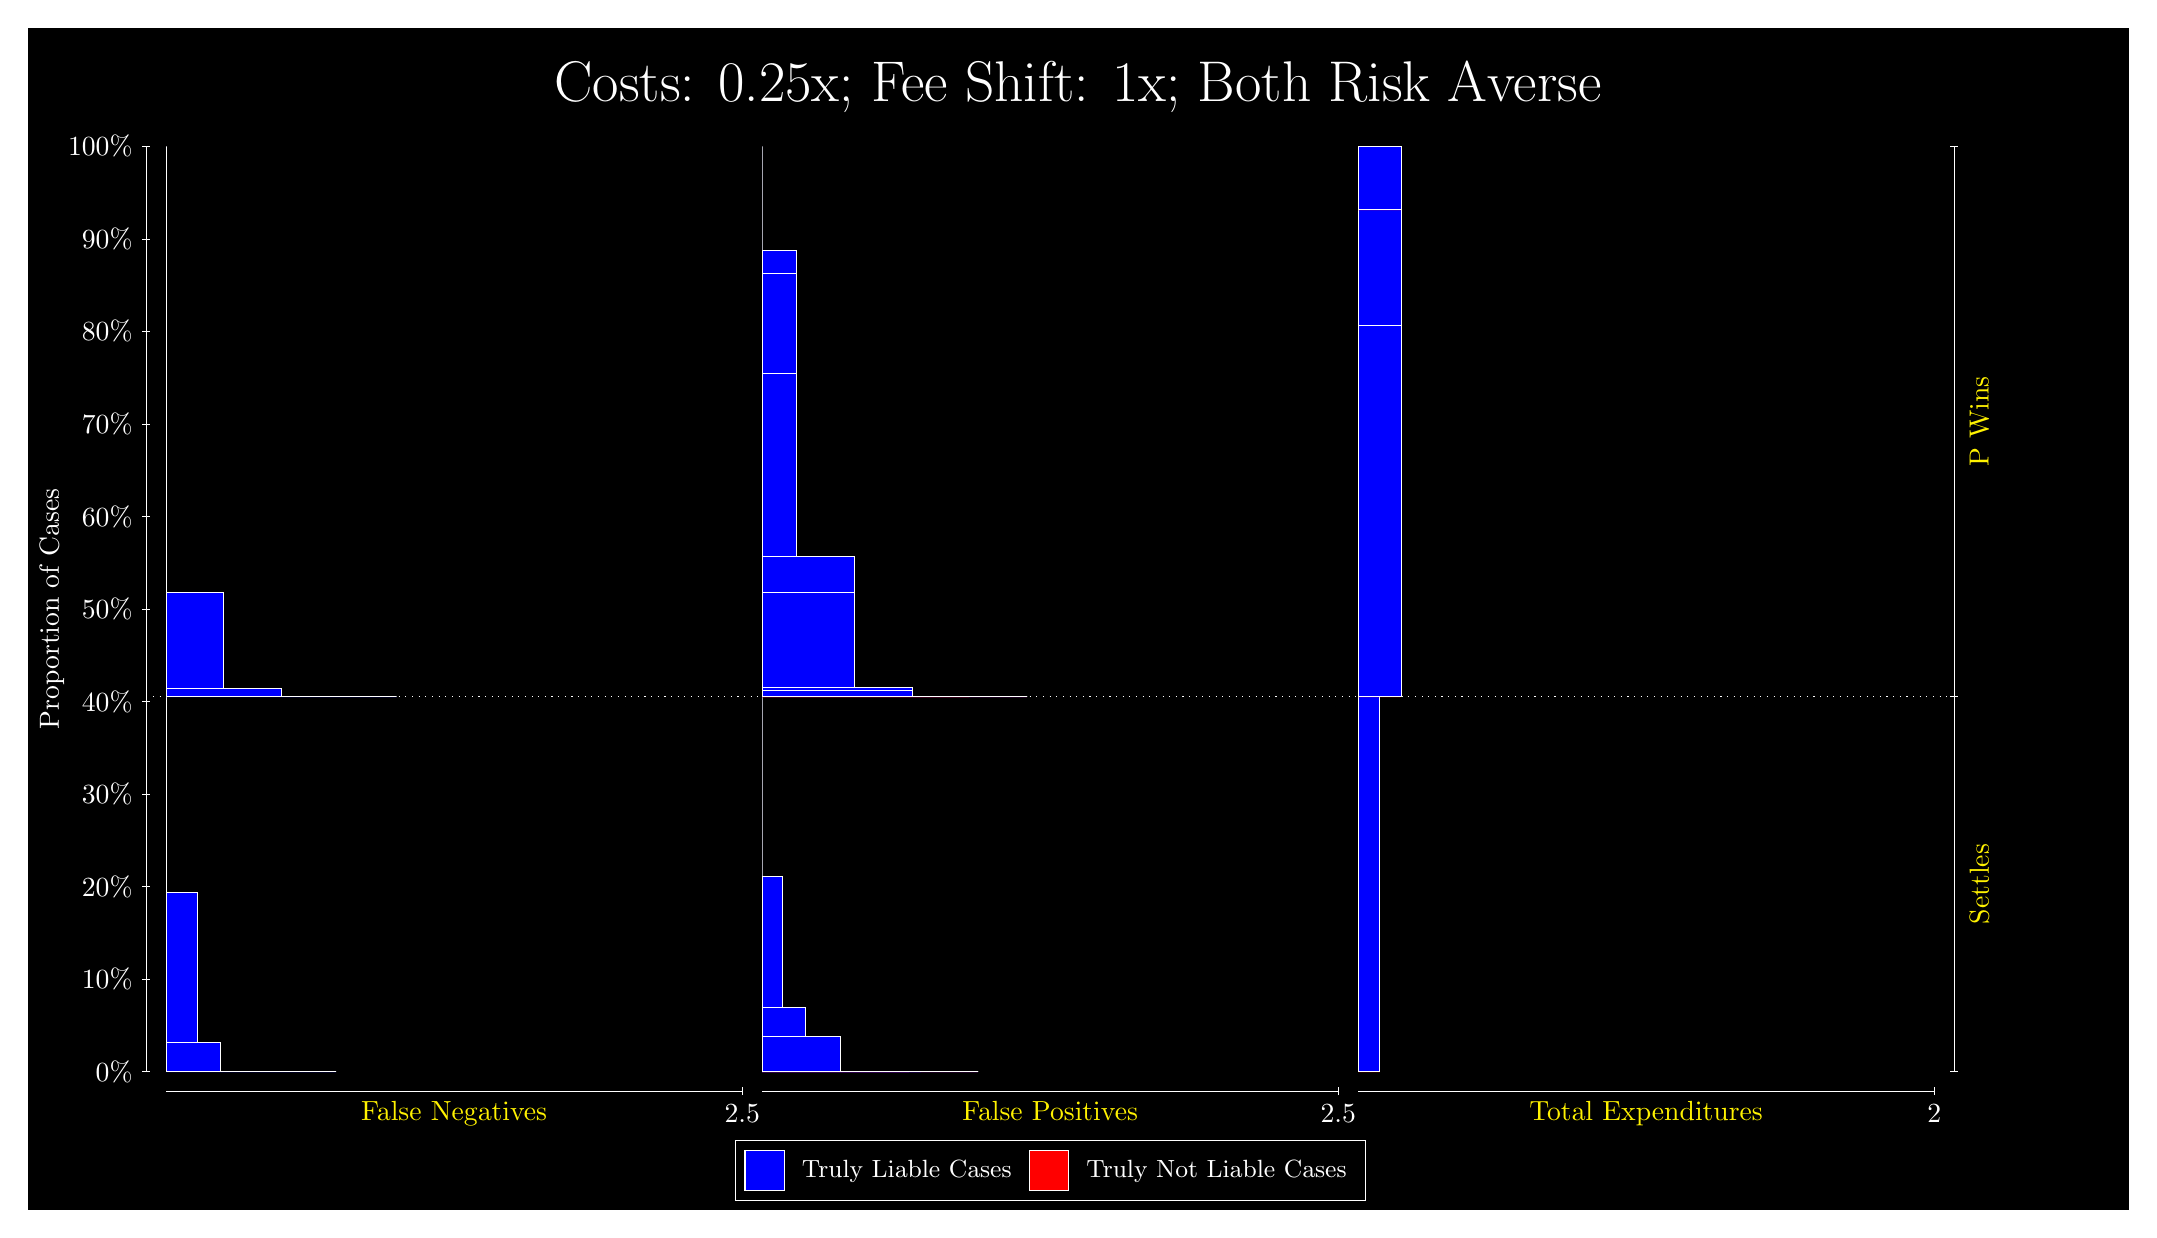
\begin{tikzpicture}
\draw[fill=black] (0,0) rectangle (26.667,15);
\draw[text=white] (0,13.5) rectangle (26.667,15) node[midway] {\huge Costs: 0.25x; Fee Shift: 1x; Both Risk Averse};
\draw[white, very thin] (1.5,1.75) -- (1.5,13.5);
\node[rotate=90, text=white, anchor=center] at (0.3, 7.625) {Proportion of Cases};
\draw[white, very thin] (1.45,1.75) -- (1.55,1.75);
\node[text=white, anchor=east] at (1.45, 1.75) {0\%};
\draw[white, very thin] (1.45,2.925) -- (1.55,2.925);
\node[text=white, anchor=east] at (1.45, 2.925) {10\%};
\draw[white, very thin] (1.45,4.1) -- (1.55,4.1);
\node[text=white, anchor=east] at (1.45, 4.1) {20\%};
\draw[white, very thin] (1.45,5.275) -- (1.55,5.275);
\node[text=white, anchor=east] at (1.45, 5.275) {30\%};
\draw[white, very thin] (1.45,6.45) -- (1.55,6.45);
\node[text=white, anchor=east] at (1.45, 6.45) {40\%};
\draw[white, very thin] (1.45,7.625) -- (1.55,7.625);
\node[text=white, anchor=east] at (1.45, 7.625) {50\%};
\draw[white, very thin] (1.45,8.8) -- (1.55,8.8);
\node[text=white, anchor=east] at (1.45, 8.8) {60\%};
\draw[white, very thin] (1.45,9.975) -- (1.55,9.975);
\node[text=white, anchor=east] at (1.45, 9.975) {70\%};
\draw[white, very thin] (1.45,11.15) -- (1.55,11.15);
\node[text=white, anchor=east] at (1.45, 11.15) {80\%};
\draw[white, very thin] (1.45,12.325) -- (1.55,12.325);
\node[text=white, anchor=east] at (1.45, 12.325) {90\%};
\draw[white, very thin] (1.45,13.5) -- (1.55,13.5);
\node[text=white, anchor=east] at (1.45, 13.5) {100\%};

\draw[white, very thin] (24.457,1.75) -- (24.457,13.5);
\draw[white, very thin] (24.407,1.75) -- (24.507,1.75);
\node[anchor=west] at (24.407, 1.75) {};
\draw[white, very thin] (24.407,6.5124) -- (24.507,6.5124);
\node[anchor=west] at (24.407, 6.5124) {};
\draw[white, very thin] (24.407,13.5) -- (24.507,13.5);
\node[anchor=west] at (24.407, 13.5) {};

\draw[white, very thin, fill=blue] (1.75,1.75) rectangle (3.9091,1.75);
\draw[white, very thin, fill=blue] (1.75,1.75) rectangle (3.1772,1.7527);
\draw[white, very thin, fill=blue] (1.75,1.7527) rectangle (3.0308,1.7527);
\draw[white, very thin, fill=blue] (1.75,1.7527) rectangle (2.4453,2.1245);
\draw[white, very thin, fill=blue] (1.75,2.1245) rectangle (2.2989,2.125);
\draw[white, very thin, fill=blue] (1.75,2.125) rectangle (2.1525,4.0318);
\draw[white, very thin, fill=red] (1.75,4.0318) rectangle (1.75,4.0318);
\draw[white, very thin, fill=blue] (1.75,4.0318) rectangle (1.75,6.5124);
\draw[white, very thin, fill=blue] (1.75,6.5124) rectangle (4.6775,6.5124);
\draw[white, very thin, fill=blue] (1.75,6.5124) rectangle (3.9457,6.5136);
\draw[white, very thin, fill=blue] (1.75,6.5136) rectangle (3.2138,6.6161);
\draw[white, very thin, fill=blue] (1.75,6.6161) rectangle (2.4819,7.8322);
\draw[white, very thin, fill=red] (1.75,7.8322) rectangle (1.75,7.8322);
\draw[white, very thin, fill=blue] (1.75,7.8322) rectangle (1.75,13.5);
\draw[white, very thin, fill=red] (9.3189,1.75) rectangle (12.063,1.75);
\draw[white, very thin, fill=blue] (9.3189,1.75) rectangle (12.063,1.75);
\draw[white, very thin, fill=blue] (9.3189,1.75) rectangle (11.332,1.75);
\draw[white, very thin, fill=red] (9.3189,1.75) rectangle (11.185,1.75);
\draw[white, very thin, fill=blue] (9.3189,1.75) rectangle (11.185,1.75);
\draw[white, very thin, fill=blue] (9.3189,1.75) rectangle (10.6,1.7527);
\draw[white, very thin, fill=blue] (9.3189,1.7527) rectangle (10.453,1.7527);
\draw[white, very thin, fill=red] (9.3189,1.7527) rectangle (10.307,1.7527);
\draw[white, very thin, fill=blue] (9.3189,1.7527) rectangle (10.307,2.1951);
\draw[white, very thin, fill=blue] (9.3189,2.1951) rectangle (9.8678,2.5648);
\draw[white, very thin, fill=blue] (9.3189,2.5648) rectangle (9.7214,2.5653);
\draw[white, very thin, fill=blue] (9.3189,2.5653) rectangle (9.575,4.2306);
\draw[white, very thin, fill=blue] (9.3189,4.2306) rectangle (9.3189,6.5124);
\draw[white, very thin, fill=red] (9.3189,6.5124) rectangle (12.686,6.5124);
\draw[white, very thin, fill=blue] (9.3189,6.5124) rectangle (12.686,6.5124);
\draw[white, very thin, fill=red] (9.3189,6.5124) rectangle (11.954,6.5124);
\draw[white, very thin, fill=blue] (9.3189,6.5124) rectangle (11.954,6.5135);
\draw[white, very thin, fill=blue] (9.3189,6.5135) rectangle (11.954,6.5138);
\draw[white, very thin, fill=red] (9.3189,6.5138) rectangle (11.222,6.5138);
\draw[white, very thin, fill=blue] (9.3189,6.5138) rectangle (11.222,6.5864);
\draw[white, very thin, fill=blue] (9.3189,6.5864) rectangle (11.222,6.6306);
\draw[white, very thin, fill=red] (9.3189,6.6306) rectangle (10.49,6.6306);
\draw[white, very thin, fill=blue] (9.3189,6.6306) rectangle (10.49,7.8319);
\draw[white, very thin, fill=blue] (9.3189,7.8319) rectangle (10.49,8.2967);
\draw[white, very thin, fill=blue] (9.3189,8.2967) rectangle (9.758,10.624);
\draw[white, very thin, fill=red] (9.3189,10.624) rectangle (9.758,10.624);
\draw[white, very thin, fill=blue] (9.3189,10.624) rectangle (9.758,11.887);
\draw[white, very thin, fill=blue] (9.3189,11.887) rectangle (9.758,12.18);
\draw[white, very thin, fill=blue] (9.3189,12.18) rectangle (9.3189,13.5);
\draw[white, very thin, fill=red] (16.888,1.75) rectangle (17.162,1.75);
\draw[white, very thin, fill=blue] (16.888,1.75) rectangle (17.162,6.5124);
\draw[white, very thin, fill=red] (16.888,6.5124) rectangle (17.437,6.5124);
\draw[white, very thin, fill=blue] (16.888,6.5124) rectangle (17.437,11.228);
\draw[white, very thin, fill=red] (16.888,11.228) rectangle (17.437,11.228);
\draw[white, very thin, fill=blue] (16.888,11.228) rectangle (17.437,12.697);
\draw[white, very thin, fill=red] (16.888,12.697) rectangle (17.437,12.697);
\draw[white, very thin, fill=blue] (16.888,12.697) rectangle (17.437,13.5);
\draw[white, dotted] (1.5,6.5124) -- (24.457,6.5124);
\draw[white, very thin] (1.75,1.5) -- (9.0689,1.5);
\node[text=yellow, anchor=north] at (5.4094, 1.5) {False Negatives};
\draw[white, very thin] (9.0689,1.45) -- (9.0689,1.55);
\node[text=white, anchor=north] at (9.0689, 1.45) {2.5};

\draw[white, very thin] (9.3189,1.5) -- (16.638,1.5);
\node[text=yellow, anchor=north] at (12.978, 1.5) {False Positives};
\draw[white, very thin] (16.638,1.45) -- (16.638,1.55);
\node[text=white, anchor=north] at (16.638, 1.45) {2.5};

\draw[white, very thin] (16.888,1.5) -- (24.207,1.5);
\node[text=yellow, anchor=north] at (20.547, 1.5) {Total Expenditures};
\draw[white, very thin] (24.207,1.45) -- (24.207,1.55);
\node[text=white, anchor=north] at (24.207, 1.45) {2};

\node[text=yellow, centered, rotate=90] at (24.777, 4.1312) {Settles};
\node[text=yellow, centered, rotate=90] at (24.777, 10.006) {P Wins};

\draw (12.978300999999998,1.5) node[draw=none] (baseCoordinate) {};
\begin{scope}[align=center]
        \matrix[scale=0.5, draw=white, below=0.5cm of baseCoordinate, nodes={draw}, column sep=0.1cm]{
            \node[rectangle, draw, minimum width=0.5cm, minimum height=0.5cm, fill=blue] {}; &
            \node[draw=none, font=\small, text=white] (B) {Truly Liable Cases}; &
            \node[rectangle, draw, minimum width=0.5cm, minimum height=0.5cm, fill=red] {}; &
            \node[draw=none, font=\small, text=white] (B) {Truly Not Liable Cases}; \\
            };
\end{scope}

\end{tikzpicture}
\end{document}